% !TEX root = ../Tesis.tex
\chapter{Redes Neuronales para análisis de series de tiempo} % Write in your own chapter title
\label{cap:RN} 

Las redes neuronales artificiales (\textit{Artificial Neural Networks}) (ANNs) se han convertido en una poderosa herramienta para resolver problemas complejos que van desde el reconocimiento de patrones hasta la toma de decisiones autónoma. Inspiradas por la configuración y el funcionamiento del cerebro humano, Nos encontramos ante un modelo computacional que consiste en un tejido de nodos interconectados entre sí. 

En el sentido de las series de tiempo, son capaces de detectar relaciones complejas y no lineales entre los datos de entrada y de salida y de aprender características y dinámicas entre y directamente de ellos \cite{Marco_TSF_Att}. A diferencia de los enfoques que usan técnicas tradicionales como el modelo autorregresivo integrado de promedio móvil (\textit{autoregressive integrated moving average}) (ARIMA) o el modelo autorregresivo integrado móvil (\textit{AutoRegressive Moving Average}) (ARMA) que se basan en suposiciones lineales o estacionales entre la información de entrada y de salida \cite{CorrOancea2014} \cite{electric_ARMA_ARIMA}, las ANNs pueden aproximar funciones no lineales. También han mostrado un mejor desempeño en comparación a modelos como la regresión lineal \cite{altay2005stock}. Aunado a esto, en la literatura podemos encontrar algunos otros modelos como el caso de las maquinas de soporte vectorial (\textit{Support Vector Machines}) (SVMs) \cite{YANG202218_SVM1} \cite{parray2020time}, árboles de desición \cite{arboles1} y bosques aleatorios \cite{khan2020predicting_randomforest22} \cite{randomforest1} que han mostrado un desempeño igualmente favorable. Para fines de este proyecto, veremos si las diferentes arquitecturas de ANNs en conjunto de la DWT generará resultados igual o mejor logrados.

%Estos se organizan en capas, dentro de las cuales cada neurona recibe datos como entrada y, junto con cierta ponderación de estos a partir de pesos y sesgos, lleva a cabo una combinación lineal y aplica una función de activación a dicho resultado para generar una salida o impulso. En un sentido general, el número de capas con el que cuenta una red es indistinto, pero siempre se puede identificar una capa de entrada, que es aquella por donde son consumidos los datos, una de salida, de donde se obtiene el resultado del procesamiento en la red y un número arbitrario de capas ocultas. 



\section{Redes Neuronales Artificiales}
Como se mencionó arriba, son un modelo de procesamiento masivo y paralelo, compuesto de neuronas conectadas entre sí con la capacidad de almacenar 'experiencia' a través del aprendizaje. A continuación se profundizará más sobre esto último. 

La unidad básica de una red neuronal es el perceptron: un combinador lineal que recibe varias entradas númericas en conjunto con un valor inmutable llamado sesgo, que pondera con cierto peso y las suma. Todo esto seguido por una función de activación que genera una respuesta o estimulo para las unidades en las siguientes capas.

\[
y = f\left(\sum_{i=1}^{n} w_i x_i + b\right)
\]

Donde:
\begin{itemize}
    \item $x_i$ es entrada $i$-ésima de la neurona.
    \item $w_i$ es el peso asociado a la entrada $x_i$ de la neurona.
    \item $b$ es el sesgo de la neurona.
    \item $f$ es una función de activación no lineal diferenciable.
\end{itemize}

La estructura de una red neuronal comprende una capa de entrada, una o más capas ocultas y una capa de salida. En cada una de ellas se encuentran cierto número de neuronas conectadas con las de la capa anterior y siguiente. Estas se comunican 'propagando hacia adelante' la información que se recibe hasta generar una respuesta por parte del modelo. Esto ocurre mediante las entradas de las unidades en capas sucesivas que reciben los impulsos de las anteriores. 

El peso ligado a cada una de las entradas de cada neurona regula qué tan importante es dicha entrada para esta, a menor peso, dicha entrada se involucrará menos en el computo de una respuesta y lo mismo en caso contrario. Así, al regular estos parámetros podemos controlar qué respuesta se genera el modelo al ser 'alimentado' por alguna entrada. Esto es especialmente conveniente para que una red nos sea útil, de esta manera se construye el aprendizaje de la red hasta obtener un modelo que cumpla la tarea para el cual fue creado. Para esto existe la etapa de entrenamiento. Durante este proceso los pesos de las conexiones entre nodos y sus sesgos se ajustan utilizando algoritmos de optimización.

\section{Entrenamiento de una Red Neuronal}

La capacidad de predicción en una red neuronal esta ligada fuertemente a qué ha aprendido de los datos, esto sucede gracias al entrenamiento empleado en esta. Este procedimiento se compone de dos partes fundamentales: el paso de propagación hacia adelante (\textit{feedforward}) y el paso de retro-propagación (\textit{backpropagation}).

El primer paso, \textbf{propagación hacia adelante}, se encarga de evaluar la señal $x_t$ en la red, siendo propagada a través de esta, capa por capa. Cada neurona calcula la suma ponderada y pasa la respuesta a la función de activación correspondiente, esta es la entrada para las neuronas de la siguiente capa. 

Cuando la propagación termina, la salida generada por la red a partir de esa entrada, llamémosle $\hat{y}_t$, se compara con el valor que esperábamos con dicha entrada, digamos $y_t$. Esro sucede a partir de la función de error $E$, que nos permite medir qué tan cerca se encuentra la predicción del valor real y así evaluar el desempeño actual de la red. Podemos encontrar funciones de error como el Error Cuadrático Medio (\textit{Mean Square Error}) (MSE), que emplearemos más adelante o el Error Absoluto Medio (\textit{Mean Absolute Error}) (MAE):
%Entropía Cruzada (\textit{Cross-Entropy})

\[ \text{MSE} = \frac{1}{n} \sum_{i=1}^{n} (y_i - \hat{y}_i)^2
\]

\[\text{MAE} = \frac{1}{n} \sum_{i=1}^{n} |y_i - \hat{y}_i|\]

%\[ \text{Entropía Cruzada} = -\sum_{i=1}^{n} y_i \log(\hat{y}_i)\]

Conociendo el error, es cuando la \textbf{retro-propagación} actúa. Se encarga de calcular los gradientes de $E$ respecto a los parámetros de la red (pesos y sesgos de todas las unidades que la componen). Para ello hacemos uso de la regla de la cadena (\textit{chain rule}) \cite{understanding_backpropagation_Kostadinov}. Sea $w_{i,j}^{c}$ un solo peso de conexión entre las neuronas $i, j$ de las capas $c-1$ oculta y $c$ de salida respectivamente, $b_{j}^{c}$ el sesgo de $j$, $a_i^{c-1}$ es la salida de la función de activación de la capa anterior y $f_j(z^c_j)$ es la señal de $j$ \footnote{Nótese que $f_j(z^c_j)$ se puede ver como $a_j^{c}$} como se puede ver en la Figura~\ref{fig:Feed-forward}.

\begin{figure}[H]
    \centering
    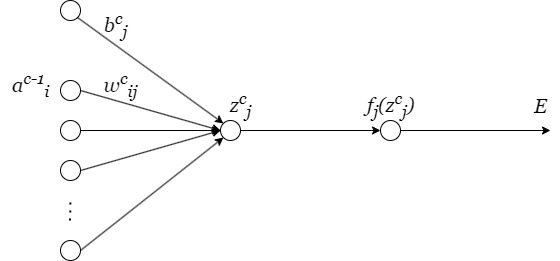
\includegraphics[width=0.8\textwidth]{Figuras/redes_neuronales/Forward_neurona.jpg}
    \caption{Esquema de la propagación hacia adelante en una neurona de salida} 
    \label{fig:Feed-forward}
\end{figure}

Se tiene entonces que los gradientes de $E$ respecto a los parámetros de la neurona son \footnote{Según las derivaciones mostradas por Haykin, S. y por Hertz, J.A., Palmer, R.G., Krogh, A. \cite{haykin2008neural} \cite{hertz1991introduction}}:

\begin{center}
    $\dfrac{\partial E}{\partial w_{i,j}^{c}} = \dfrac{\partial E}{\partial z_{j}^{c}}a_i^{c-1}$
\end{center}

Y también respecto a algún sesgo en $c$:

\begin{center}
    $\dfrac{\partial E}{\partial b^c_j} = \dfrac{\partial E}{\partial z_{j}^{c}}$
\end{center}

Donde el termino de gradiente local en neuronas de capas de salida:

\begin{center}
    $\dfrac{\partial E}{\partial z_{j}^{c}} = E f'(z^c_j)$
\end{center}

Debido a que las neuronas de capas ocultas no cuentan con una salida esperada, esta debe de ser determinada recursivamente en términos de las salidas esperadas de las unidades en las capas sucesivas. De esta forma es en la que el cálculo del gradiente se efectúa para estas, dependiendo de los gradientes de las neuronas a las cuales esta se conecta y a su vez, el obtener el gradiente de unidades en capas anteriores es mediante el gradiente calculado de esta última neurona. Es así que la retro-propagación de los gradientes de los parámetros de la red actúa.

Sea entonces $c$ una capa oculta y $c+1$ es la capa de salida y $k$ es una neurona a elegir en el conjunto de las unidades para las cuales $j$ tiene una salida:

\begin{figure}[H]
    \centering
    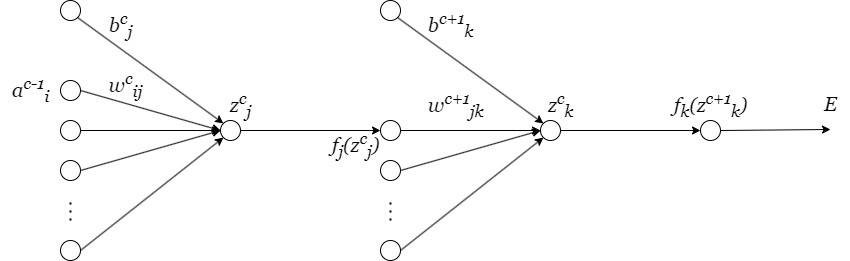
\includegraphics[width=0.8\textwidth]{Figuras/redes_neuronales/Feed-forward 2 neuronas.jpg}
    \caption{Esquema de la propagación hacia adelante en una neurona en una capa oculta conectada a una neurona de salida} 
    \label{fig:Feed-forward2}
\end{figure}

Así, el gradiente local de $j$:

\[
\dfrac{\partial E}{\partial z_{j}^{c}} = f'(z^c_j)\sum_{k} \dfrac{\partial E}{\partial z_{k}^{c+1}} w^{c+1}_{jk}
\]

Con los gradientes calculados, el algoritmo de optimización aplica una estrategia para ajustar los pesos de las conexiones en la red y los sesgos de cada neurona para minimizar la diferencia entre la salida que obtuvimos de esta y los valores originales. Algunos ejemplos de algoritmos de optimización más comúnmente usados son Descenso por el Gradiente (\textit{Gradient Descent}) (GD), Descenso por el Gradiente Estocástico (\textit{Stochastic Gradient Descent}) (SGD), Estimación Adaptativa de Momento (\textit{Adaptative Moment Estimation}) (ADAM) y Levenberg-Marquardt (LM). A continuación profundizaremos sobre estos. 

\subsection{Algoritmos de Optimización}

\begin{itemize}
    \item \textbf{Descenso por el gradiente}
    Es el método más común para minimizar $E$. Ajusta los pesos y sesgos en la dirección opuesta al gradiente multiplicado por la tasa de aprendizaje (\textit{learning rate}) (debido a que el gradiente indica la dirección hacia donde crece la función o donde se encuentra un máximo local).
    Este proceso se repite iterativamente durante varias épocas \footnote{Una época comprende una iteración del proceso completo de entrenamiento, es decir propagación hacia adelante, cálculo en $E$, retro-propagación y algoritmo de optimización.}, hasta que la función de pérdida converge o se detiene según algún criterio predefinido.

    Así entonces, las actualizaciones de cada peso y sesgo está dado por:

\begin{center}
    $w_{ij}^{c} := w_{ij}^{c} - \alpha \dfrac{\partial E}{\partial z_{j}^{(c)}}a_i^{c-1}$

    $b^c_j := b^c_j - \alpha \dfrac{\partial E}{\partial z_{j}^{(c)}}$
\end{center}

    \item \textbf{SGD}
    Es una variante específica del Descenso por el Gradiente.
    En vez de calcular el gradiente utilizando todo el conjunto de datos de entrenamiento, se obtiene utilizando solo un subconjunto de los datos (mini lotes\footnote{\textit{mini batch}}) seleccionado de manera aleatoria en cada iteración del entrenamiento ayudando a evitar mínimos locales y puntos de estancamiento durante el entrenamiento. Esto hace que el cálculo del gradiente sea más eficiente, especialmente para conjuntos de datos grandes.
    
    \item \textbf{ADAM}
    Es un optimizador que combina la idea del descenso por el gradiente con el movimiento promedio de los momentos. Utiliza estimaciones adaptativas del primer y segundo momento de los gradientes para ajustar la tasa de aprendizaje de forma individual para cada parámetro de la red, lo que lo hace especialmente útil en problemas con características de datos variables o no estacionarias. \cite{adam_kingma}
    Además esto permite que, durante la optimización de la función de error ADAM da 'pasos' conforme al comportamiento del gradiente en ese instante, alcanzando el mínimo de manera más precisa. 

    ADAM emplea dos arreglos del tamaño de los parámetros de la red que se encargarán de contener el movimiento promedio o media móvil del primer y segundo momento de los gradientes, estos son actualizados en cada iteración del algoritmo ponderando los gradientes y el cuadrado de este respectivamente junto con $m_{t-1}$ y $v_{t-1}$, los vectores de la corrida anterior (linea 4 y 5). Finalmente se actualizan los parámetros $x_t$ (linea 7) con los vectores cuando se encuentran corregidos a partir de la taza de decaimiento (linea 6), esto para evitar un sesgo en la inicialización en cero.
    
    . %También incluye un término de momentum que ayuda a acelerar la convergencia y suaviza las actualizaciones de los pesos.

    \begin{algorithm}[H]
        \caption{Algoritmo de Optimización ADAM}
        \KwIn{Conjunto de datos $X$, tasa de aprendizaje $\alpha$, $\beta_1$, $\beta_2$, $\epsilon$}
        \SetAlgoLined
        \SetKwComment{Comment}{\% }{}
        \SetKwInOut{Input}{Entrada}
        \SetKwInOut{Output}{Salida}
        \Input{Parámetros del modelo: $x_0$}
        \Input{Momentos de primer y segundo orden: $m_0 = 0$, $v_0 = 0$}
        \Input{Contador de iteraciones: $t = 0$}
        \BlankLine
        \While{no se alcance el criterio de parada}{
            $t \gets t + 1$\;
            Calcular el gradiente: $g_t = \nabla_x E(x_{t-1})$\;
            Actualizar el momento de primer orden: $m_t = \beta_1 m_{t-1} + (1 - \beta_1) g_t$\;
            Actualizar el momento de segundo orden: $v_t = \beta_2 v_{t-1} + (1 - \beta_2) g_t^2$\;
            Corregir los momentos de primer y segundo orden: $\hat{m}_t = \frac{m_t}{1 - \beta_1^t}$, $\hat{v}_t = \frac{v_t}{1 - \beta_2^t}$\;
            Actualizar los parámetros: $x_t = x_{t-1} - \alpha \frac{\hat{m}_t}{\sqrt{\hat{v}_t} + \epsilon}$\;
        }
        \Output{Parámetros del modelo $x_t$}
    \end{algorithm}
    
    \item \textbf{Levenberg Marquardt (LM)}
    Es un algoritmo de optimización no lineal utilizado principalmente en problemas de ajuste de curvas y regresión no lineal. A diferencia de los métodos basados únicamente en el gradiente, LM utiliza una estrategia de optimización iterativa que combina técnicas de descenso por el gradiente y gauss-newton. El algoritmo ajusta los parámetros de manera iterativa, utilizando una matriz de aproximación o la misma matriz hessiana en combinación con el gradiente para guiar la búsqueda hacia el mínimo local de la función de error.
    La dirección de búsqueda del algoritmo se define como sigue:

    \begin{center}
    $\Delta x = -[H + \lambda I] ^{-1} \nabla E(x)$
    \end{center}

    Donde:
    \begin{itemize}
        \item $x$ son los parámetros de la red.
        \item $E(x)$ es la función de error.
        \item $H$ es la matriz Hesiana de $E(x)$.
    \end{itemize}

    \begin{algorithm}
        \caption{Algoritmo de Levenberg-Marquardt}
        \KwData{Función de error $E(x)$, punto inicial $x_0$, parámetros de ajuste $\lambda_0$, tolerancia $\epsilon$}
        \KwResult{Solución $\mathbf{x}^*$}
        Inicializar $x \leftarrow x_0$\;
        Inicializar $\lambda \leftarrow \lambda_0$\;
        Definir $\epsilon_1 \leftarrow$ Tolerancia para la convergencia del método\;
        Definir $\epsilon_2 \leftarrow$ Tolerancia para el valor del gradiente\;
        \Repeat{convergencia}{
            Calcular el vector de gradiente $\nabla E(x)$\;
            Calcular la matriz Hessiana $H$\;
            Calcular el paso de Levenberg-Marquardt: $\Delta \mathbf{x} = -[H + \lambda I]^{-1} \nabla E(x)$\;
            Calcular el valor de la función de error con el paso propuesto: $f_{\text{prop}} = f(\mathbf{x} + \Delta \mathbf{x})$\;
            Calcular el valor de la función de error en el punto actual: $f_{\text{actual}} = f(\mathbf{x})$\;
            \If{$f_{\text{prop}} < f_{\text{actual}}$}{
                Aceptar el paso: $\mathbf{x} \leftarrow \mathbf{x} + \Delta \mathbf{x}$\;
                Actualizar $\lambda$: $\lambda \leftarrow \frac{\lambda}{2}$\;
            }
            \Else{
                Rechazar el paso: No actualizar $\mathbf{x}$\;
                Aumentar $\lambda$: $\lambda \leftarrow 2\lambda$\;
            }
            \If{$|$ $f_{\text{prop}} - f_{\text{actual}}$ $|$ $> \epsilon_1$ o $|| \nabla E(x)|| > \epsilon_2$}{
                Detener el algoritmo\;
            }
        }
        \end{algorithm}

    
\end{itemize}

    A pesar de ser un método efectivo, LM no es un algoritmo tan usado como SGD o ADAM debido a que es computacionalmente costoso, debido al calculo de la matriz hessiana o su aproximación. 
    

\newpage

\section{Redes Neuronales Auto-regresivas}

Las ARNNs, o redes neuronales auto-regresivas (\textit{Autorregresive Neural Networks} también llamadas NARNN (por \textit{Not linear Autorregresive Neural Networks}), se emplean en el estudio de series temporales y en tareas de predicción secuencial. Se trata de un tipo específico de arquitectura de redes neuronales que consiste en predecir los valores futuros a partir de los pasados $d$ valores, contemplando la idea de que el comportamiento en el pasado de una serie temporal tiene impacto en su desempeño en el futuro. Buscan estimar $p(x_{t} | x_{t-1}, ..., x_1)$

Dada una serie temporal $\{ x_1, x_2, \ldots, x_t \}$, donde $x_i$ representa una muestra en el tiempo $i$, una ARN puede predecir el valor futuro $\hat{x}_{t+1}$ basado en las observaciones pasadas $x_{t-1}, x_{t-2}, \ldots, x_{t-d}$, con $t,d \in \mathbb{N} $ 

Una ARN puede expresarse como una función $f$ que mapea las observaciones pasadas a la predicción futura:

\[
\hat{x}_{t} = f(x_{t-1}, x_{t-2}, \ldots, x_{t-d})
\]

En la práctica, las ARN suelen tener una estructura recurrente \footnote{Según Haykin, podemos interpretar a una ARN como una Red Neuronal Recurrente en si misma, sin embargo para fines de este trabajo, trataremos a ambas como entidades independientes.} (que trataremos más adelante), hecho que no implica el desuso de arquitecturas básicas con propagación hacia adelante (\textit{feedforward}) como unidad base. 

\begin{figure}[h]
    \centering
    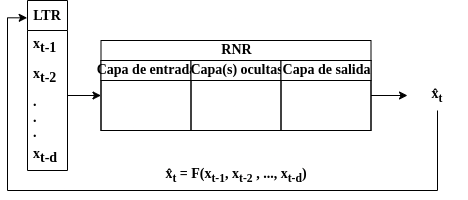
\includegraphics[width=0.5\textwidth]{Figuras/redes_neuronales/NARNN_diagrama.png}
    \caption{Esquema general de una RNN} 
    \label{fig:rRNN_diagrama}
\end{figure}

Sin embargo, implementar capas recurrentes permite que la red capture dependencias o relaciones implícitas a lo largo de la serie temporal y realice predicciones aun más precisas (como también veremos más adelante). Las ARN también pueden incorporar capas convolucionales o capas completamente conectadas, dependiendo de la naturaleza de los datos y la complejidad del problema de predicción. 

\section{Redes Neuronales Recurrentes}

Las Redes Neuronales Recurrentes (\textit{Recurrent Neural Networks}) (RNNs) son un sistema dinámico no lineal. A diferencia de las redes neuronales tradicionales, las RNN tienen conexiones retro-alimentadas, lo que significa que las salidas de algunos de sus nodos se incluyan como parte de la entrada de los mismos en siguientes iteraciones del proceso de predicción y la información que fluye a través de éstas pueda hacerlo cíclicamente. Esto permite retener y aprovechar información sobre estados anteriores a lo largo de la secuencia de datos (persistencia). Están diseñadas para modelar datos secuenciales, como palabras en un texto o muestras en una serie temporal cuyos datos en cierto espacio de tiempo $\delta t$ guardan relación con algún intervalo $\delta (t-d)$ en el pasado. 

Dada una secuencia de entrada $\{ x_1, x_2, \ldots, x_t \}$%, y una secuencia de salida correspondiente $\{ y_1, y_2, \ldots, y_t \}$, 
una RNN se define de forma general como sigue:

\[ h_t = f(W \cdot [x_t, h_{t-1}] + b) \]
\[ o_t = g(h_t) \]

Donde:
\begin{itemize}
    \item $h_t$ es el estado oculto o estado interno en el tiempo $t$. Representa la memoria de la red en ese momento y se calcula utilizando una función de activación $f$ que toma como entrada el elemento actual $x_t$ y el estado oculto anterior $h_{t-1}$.
    \item $o_t$ es la salida de la red en el tiempo $t$, calculada utilizando una función de activación $g$ aplicada al estado oculto $h_t$ \footnote{También se suele ver a $g=f$ de manera que $o_t = h_t$.}.
    \item $f$ y $g$ son funciones de activación no lineales, como la función sigmoide ($\sigma$) o la función tangente hiperbólica ($tanh$), que introducen la no linealidad en el modelo y permiten a la red capturar relaciones complejas en los datos secuenciales.
\end{itemize}

Una de las arquitecturas más simples de las RNNs son los Perceptrones Multicapa Recurrentes (\textit{Recurrent Multilayer Perceptron}) RMLP que se caracteriza porque las neuronas de cada una de sus capas recibe como parte de su entrada el valor de salida que esta misma genero en la iteración anterior, es decir, a salida de una capa en un tiempo $t$ puede ser una función de su salida en el tiempo $t-1$, además de la entrada actual. Se define como sigue:

\[x_{I,n+1} = \Psi_I(x_{I,n},U_{n})\]
\[x_{II,n+1} = \Psi_{II}(x_{II,n},x_{I,n+1})\]
\begin{center}
.\\
.\\
.\\  
\end{center}

\[x_{o,n+1} = \Psi_o(x_{o,n},x_{M,n+1})\]

A pesar de que las RNNs hacen uso de información en el pasado para modelar el comportamiento actual, la manera cíclica de actuar de éstas sólo influye cuando los datos que necesitamos pertenecen al pasado inmediato anterior de la predicción actual. Si por el contrario, lo que intentamos predecir está ligado a muestras que se presentaron con mayor anterioridad, la red perderá su capacidad de predicción con base a esta información. Es aquí donde se nos presenta el llamado problema de Dependencias a Largo Plazo  (\textit{Long-term dependencies}) \cite{understanding_lstm_Olah}. 

\subsection{Retro-propagación a través del tiempo}

Se trata de una extensión del algoritmo de retro-propagación util para el ajuste de parámetros en una red recurrente.

En principio, se usa la técnica de desdoblamiento que menciona Haykin, S.: \cite{haykin2008neural} el modelo recurrente representa sus múltiples pasos en el tiempo a través de una red neuronal de propagación hacia adelante:

\begin{enumerate}
    \item Para cada paso temporal en $(t_0,t]$ la red de propagación hacia adelante, llamémosle $F$, tiene una capa con N neuronas, que es el número total de unidades en la red recurrente $R$.

    \item Para cada paso temporal, existe una conexión de la neurona $i$ de la capa $c$ a la neurona $j$ en la capa $c+1$ 
\end{enumerate}

El conjunto de datos que se usará para entrenamiento se particionará en intervalos temporales llamados épocas. Sea $t_0$ y $t_1$ el tiempo de inicio y fin de cierta época. La función de error total de la salida de la red:

\[
E_{total} = \sum^{t_1}_{n=n_0}\sum_{i}E_{i,t}
\]

Donde:
\begin{itemize}
    \item $i$ es el conjunto de neuronas de la red
    \item $E_{i,t}$ es el error de la salida esperada de $i$
\end{itemize}

Así, el algoritmo de retro-propagación a través del tiempo se define como sigue:

\begin{enumerate}
    \item Se realiza el paso de la propagación hacia adelante y se asegura el estado de la red (se guardan sus parámetros).
    \item Se realiza el paso de la retro-propagación:

    \[
    \dfrac{\partial E_{total}}{\partial v_{i,t}} = \left\{
    \begin{array}{ll}
    \varphi'(v_{i,t})E_{i,t} & \text{si } t > t_1 \\
    \varphi'(v_{i,t}) \left[E_{i,t}+\sum_{j}w_{ij}\dfrac{\partial E_{total}}{\partial v_{j,t+1}}\right] & \text{si } t_0 < t < t_1
\end{array}
\right.
    \]
    
    Donde:
    \begin{itemize}
        \item $\varphi'(\cdot)$ es la derivada de la función de activación.
        \item $v_{i,t}$ es el estado de la neurona $i$ en el tiempo $t$
    \end{itemize}

    Así las iteraciones sobre la formula actúan desde el tiempo $t_1$ hasta $t_0$.
    
    \item Una vez concluida la retro-propagación, se realiza el ajuste de pesos correspondiente, según el algoritmo de optimización elegido. 

    \[
    w_{ij} := w_{ij} - \alpha \dfrac{\partial E_{total}}{\partial w_{ij}}
    \]

    Y:
    \[
    \dfrac{\partial E_{total}}{\partial w_{ij}} = -\sum^{t_1}_{t=t_0+1}\dfrac{\partial E_{total}}{\partial v_{i,t}}x_{j,t-1}
    \]

    Donde:
    \begin{itemize}
        \item $x_{j,t-1}$ es la entrada aplicada a la $j$-ésima conexión de la neurona $i$ en el tiempo $t-1$.
    \end{itemize}
    
\end{enumerate}

\subsection{Redes Neuronales LSTM}

Las redes neuronales con células de Memoria de Corto y Largo Plazo o LSTM (\textit{Long Short-Term Memory}) son un tipo especializado de RNNs, presentadas por primera vez por Hochreiter y Schmidhube (1991) \cite{LSTM}, diseñadas para manejar con mayor eficacia los problemas de dependencias entre datos secuenciales. Las LSTM tienen unidades de memoria llamadas ''células de memoria'' que les permiten retener y actualizar información durante largos períodos, a diferencia de las RNNs comunes.

La idea central de una célula LSTM es su estado(\textit{cell state}) y sus diferentes compuertas. La primera actúa como una banda transportadora o autopista que transfiere información a lo largo de la cadena de secuencia de la célula, mientras que las compuertas actúan como redes neuronales con la capacidad de aprender qué información se olvidará o recordará en iteraciones siguientes.  Dada una secuencia de entrada $\{ x_1, x_2, \ldots, x_t \}$ y una secuencia de salida correspondiente $\{ y_1, y_2, \ldots, y_t \}$, una célula de memoria LSTM realiza la siguiente operación:

\[ i_t = \sigma(W_{i} \cdot [x_t, h_{t-1}] + b_i) \]
\[ f_t = \sigma(W_{f} \cdot [x_t, h_{t-1}] + b_f) \]
\[ g_t = \tanh(W_{g} \cdot [x_t, h_{t-1}] + b_g) \]
\[ C_t = f_t \odot C_{t-1} + i_t \odot g_t \]
\[ o_t = \sigma(W_{o} \cdot [x_t, h_{t-1}] + b_o) \]
\[ h_t = o_t \odot tanh(C_t) \]

Donde:
\begin{itemize}
    \item $i_t$, compuerta de entrada (\textit{input gate}): determina qué valores serán los candidatos para formar parte del nuevo estado de la célula $C_t$.
    \item $f_t$, compuerta de olvido (\textit{forget gate}): mediante la función sigmoide se decide que datos olvidar (0) o mantener (1) del estado oculto (\textit{hidden state}) anterior $h_{t-1}$.
    \item $g_t$ es la candidata de celda.
    \item $C_t$ es el estado de la célula en el tiempo $t$, que almacena y actualiza la información relevante a largo plazo. Se obtiene al multiplicar $g_t$ por $f_t$ obteniendo los valores candidatos omitiendo aquellos que se decidieron olvidar, al sumar $i_t \cdot g_t$ tenemos todas las actualizaciones de los valores de $C_t$.
    \item $o_t$ compuerta de salida (\textit{output gate}).
    \item $h_t$ es el estado oculto en el tiempo $t$, que se calcula utilizando una versión filtrada del estado de la célula.
\end{itemize}

\begin{figure}[h]
    \centering
    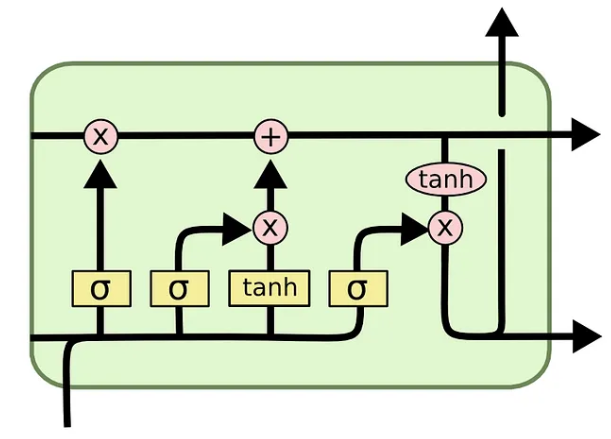
\includegraphics[width=0.5\textwidth]{Figuras/redes_neuronales/diagrama_celda_LSTM.png}
    \caption{Esquema general de una célula LSTM (Recuperado de \cite{understanding_lstm_Olah}).} 
    \label{fig:diagrama_LSTM}
\end{figure}

%Aunado al hecho que las redes neuronales con células LSTM resulven el problema de las Dependencias de Termino largo, esta arquitectura fue ideada para solventar el problema del gradiente desvaneciente (\textit{Vanishing Gradient}). El problema del gradiente desvaneciente es una limitación que puede surgir durante el entrenamiento de redes neuronales profundas, especialmente aquellas con muchas capas. Se manifiesta cuando los gradientes calculados durante el proceso de retropropagación disminuyen exponencialmente a medida que se propagan hacia atrás a través de las capas de la red. Se vuelve problemático porque los pesos de las capas iniciales de la red apenas se actualizan durante el entrenamiento, lo que significa que estas capas aprenden muy lentamente o incluso no aprenden en absoluto. Como resultado, las capas posteriores de la red pueden recibir poca o ninguna información útil de las capas anteriores, lo que dificulta el aprendizaje efectivo de la red en su conjunto.

\subsubsection{Entrenamiento de una red LSTM}

El entrenamiento de una red con células LSTM parte del mismo principio que el de un perceptrón multicapa: un paso de propagación hacia adelante, evaluación del error por medio de la función $E$, la retro-propagación con el cálculo de sus respectivos gradientes y la optimización según el algoritmo que se aplique.

Para obtener los gradientes de $E$ con respecto de cada uno de los componentes con ayuda de la regla de la cadena. Por ejemplo, se sabe que durante la propagación hacia adelante el flujo de la información de $o_t$:

\begin{center}
    $o_t$ a $E$: $o_t \longrightarrow h_t \longrightarrow E$
\end{center}
Por lo que el cálculo del respectivo gradiente es:

$\dfrac{E}{o_t} = \dfrac{\partial E}{\partial h_t} \cdot \tanh(c_t)$

Y para $a_o = W_{o} \cdot [x_t, h_{t-1}] + b_o$:

\begin{center}
    $a_o$ a $E$: $a_t \longrightarrow o_t \longrightarrow h_t \longrightarrow E$
\end{center}

Y entonces:

$\dfrac{E}{\partial a_o} = \dfrac{\partial E}{\partial h_t} \cdot \tanh(c_t) \cdot o_t(1-o_t)$ \footnote{El desarrollo de los anteriores se puede ver reflejado en \ref{ApA}.}

Y consecuentemente para los demás compuertas de la célula \cite{LSTM_gradients_Rahuljha} \footnote{Aquí podemos encontrar la derivación completa de cada una de las compuertas.} \cite{LSTM_fbp_calc_grad_Mallya}

Los gradientes de la célula LSTM:

\begin{center}
    $\dfrac{\partial E}{h_t} = y_t - h_t$ \footnote{Solo si se usa a $E = ECM(y_t,h_t)$.}
    
    $\dfrac{\partial E}{\partial o_t} = \dfrac{\partial E}{\partial h_t} \cdot tanh(C_t)$

    $\dfrac{E}{\partial a_o} = \dfrac{\partial E}{\partial h_t} \cdot \tanh(c_t) \cdot o_t(1-o_t)$ 

    $\dfrac{\partial E}{\partial C_t} = \dfrac{\partial E}{\partial h_t} \cdot o_t \cdot (1-tanh^2(C_t))$

    $\dfrac{\partial E}{\partial g_t} = \dfrac{\partial E}{\partial C_t} \cdot i_t$

    $\dfrac{E}{\partial a_C} = \dfrac{\partial E}{\partial C_t} \cdot i_t \cdot (1-g_t^2)$ 

    $\dfrac{\partial E}{\partial i_t} = \dfrac{\partial E}{\partial C_t} \cdot g_t$

    $\dfrac{E}{\partial a_i} = \dfrac{\partial E}{\partial C_t} \cdot g_t \cdot i_t(1-i_t)$ 

    $\dfrac{\partial E}{\partial f_t} = \dfrac{\partial E}{\partial C_t} \cdot C_{t-1}$

    $\dfrac{E}{\partial a_f} = \dfrac{\partial E}{\partial C_t} \cdot C_{t-1} \cdot f_t(1-f_t)$ 

    $\dfrac{E}{\partial C_{t-1}} = \dfrac{\partial E}{\partial C_t} \cdot f_t$ 
\end{center}

Definimos $Z_t = [x_t, h_{t-1}]$. Durante la propagación hacia adelante $Z_t$ tiene flujo por medio de las compuertas de entrada, salida, de olvido y el estado de la célula:

\begin{center}
    $\dfrac{\partial E}{\partial Z_t} = W_f^T\dfrac{\partial E}{\partial a_f} + W_i^T\dfrac{\partial E}{\partial a_i} + W_o^T\dfrac{\partial E}{\partial a_o} + W_C^T\dfrac{\partial E}{\partial a_C}$
\end{center}

Por último, para los pesos y sesgos:

\begin{center}
    $\dfrac{\partial E}{W_t} = \dfrac{\partial E}{\partial a_f} \cdot z_t^T$, 
    $\dfrac{\partial E}{b_t} = \dfrac{\partial E}{\partial a_f}$

    $\dfrac{\partial E}{W_i} = \dfrac{\partial E}{\partial a_i} \cdot z_t^T$, 
    $\dfrac{\partial E}{b_i} = \dfrac{\partial E}{\partial a_i}$

    $\dfrac{\partial E}{W_o} = \dfrac{\partial E}{\partial a_o} \cdot z_t^T$, 
    $\dfrac{\partial E}{b_o} = \dfrac{\partial E}{\partial a_o}$
\end{center}

\subsection{Redes Neuronales GRU}

Las redes neuronales con Unidades Recurrentes Cerradas (\textit{Gated Recurrent Unis}) o GRU, propuestas por Cho, et. al \cite{GRU}, son una arquitectura de RNR diseñada para modelar y procesar eficientemente datos secuenciales. Las GRU, al igual que las LSTM, tienen como objetivo resolver el problema de las dependencias a largo plazo en datos secuenciales. No obstante, las GRU resultan más sencillas que las LSTM y poseen menos parámetros, lo cual acelera el proceso de entrenamiento y disminuye la susceptibilidad al sobreajuste en conjuntos de datos reducidos.

Una GRU consta de compuertas de actualización (\textit{update gate}) y reinicio (\textit{reset gate}) que controlan el flujo de información dentro de la unidad. Dada una secuencia de entrada $x_t$, una GRU se define a partir de las siguientes ecuaciones:

\[ z_t = \sigma(W_z \cdot x_t + U_z \cdot h_{t-1}) \]
\[ r_t = \sigma(W_r \cdot x_t + U_r \cdot h_{t-1}) \]
\[ g_t = \tanh(W_g \cdot x_t + r_t \odot U_g \cdot h_{t-1}) \]
\[ h_t = (1 - z_t) \odot g_t + z_t \odot h_{t-1} \] \footnote{También podemos encontrar la implementación $h_t = (1 - z_t) \odot h_{t-1} + z_t \odot g_t$ como podemos ver en \cite{GRU_units_in_R_Fichou}. }

Donde:
\begin{itemize}
    \item $z_t$ es la puerta de actualización, que controla cuánto de la información previa $h_{t-1}$ debe ser actualizada.
    \item $r_t$ es la puerta de reinicio, que controla cuánto de la información previa $h_{t-1}$ debe ser olvidada.
    \item $g_t$ es el candidato para el nuevo estado oculto $h_t$, que se basa en la información actual $x_t$ y el estado anterior $h_{t-1}$ ponderado por la puerta de reinicio $r_t$.
    \item $\sigma$ es la función sigmoide y $\odot$ denota la multiplicación elemento por elemento.
\end{itemize}

\begin{figure}[h]
    \centering
    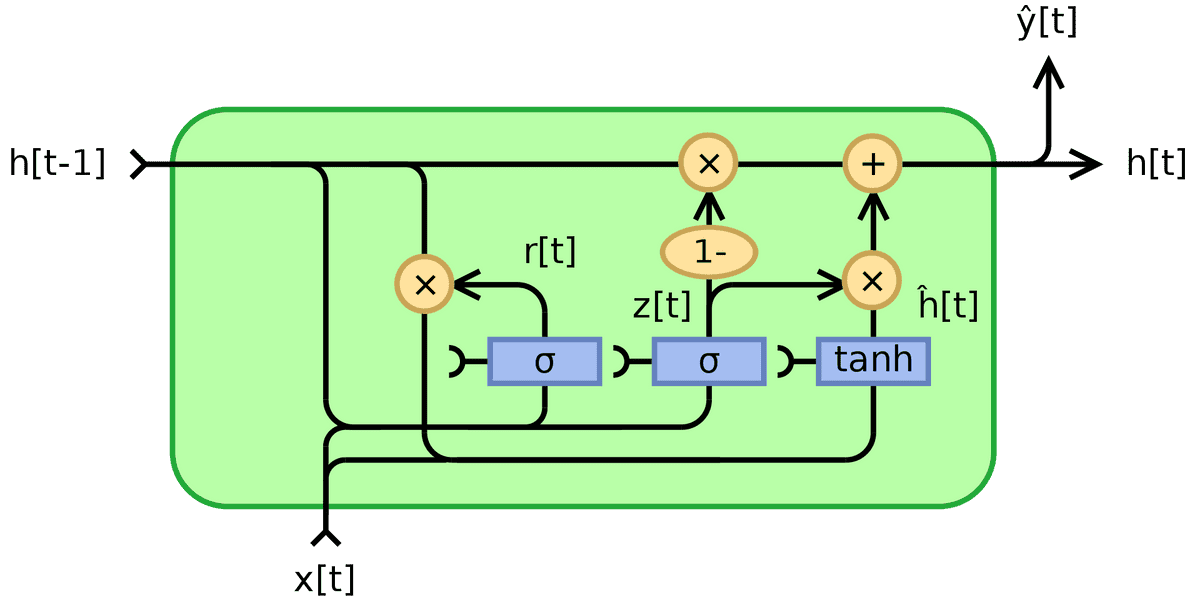
\includegraphics[width=0.5\textwidth]{Figuras/redes_neuronales/diagrama_celda_GRU.png}
    \caption{Esquema general de una célula GRU (Recuperado de Jeblad, CC BY-SA 4.0, \url{https://commons.wikimedia.org/w/index.php?curid=66234713}} 
    \label{fig:diagrama_GRU}
\end{figure}

\subsubsection{Entrenamiento de una red GRU}

En un sentido similar al desarrollo de entrenamiento de las redes LSTM, los gradientes de cada uno de los componentes de la célula son:

\begin{center}
    $\dfrac{\partial E}{g_t} = \dfrac{\partial E}{\partial h_t}(1-z_t)$
    
    $\dfrac{\partial E}{r_t} = \dfrac{\partial E}{\partial h_t}(1-z_t) W_g  h_{t-1} [1-g_t^2]$

    $\dfrac{\partial E}{z_t} = \dfrac{\partial E}{\partial h_t}(h_{t-1} - g_t)$
\end{center}

De la misma manera, los parámetros de la red quedan\footnote{Estos gradientes fueron recuperados de \cite{forward_and_Backprop_GRU_Mihir}.}:

\begin{center}
    $d1 = \dfrac{\partial E}{\partial h_t} (1-z_t) (1-g_t^2)$
    
    $d2 = [ [ ( d1 ) \odot W_h^T] h_{t-1}] (r_t(1-r_t))$

    $d3 = [h_{t-1}\dfrac{\partial E}{\partial h_t} - g_t\dfrac{\partial E}{\partial h_t}](z_t(1-z_t))$

    $\dfrac{\partial E}{W_r} = h_{t-1}^T \odot (d2)$

    $\dfrac{\partial E}{U_r} = x_t^T \odot (d2)$

    $\dfrac{\partial E}{W_z} = h_{t-1}^T \odot (d3)$

    $\dfrac{\partial E}{U_Z} = x_t^T \odot (d3)$

    $\dfrac{\partial E}{W_h} = h_{t-1}^T \odot (d1)$

    $\dfrac{\partial E}{U_h} = x_t^T \odot (d1)$
\end{center}

%problema del gradiente desvaneciente:




